\section{Experiments}
\label{sec:experiments}

The parameter space for the hidden states, the associated prior $H$ on
$\btheta$, and the similarity function
$\Phi$, is application-specific, but we consider here the case where a state
consists of a finite $D$-dimensional binary vector, $\eta_j$, the similarity
function is a Laplacian kernel defined with respect to Hamming
distance between pairs $\eta_j$ and $\eta_{j'}$, with decay parameter
$\lambda$, and the emission distribution is linear-Gaussian, with $D
\times K$ weight matrix $\bW$, so that each $K$-dimensional
observation is $\Norm{\bW \eta_j}{\Sigma}$.  For all experiments, we 
will assume that $\Sigma$ does not depend on $j$, but this assumption
is easily relaxed if appropriate.  For finite-length binary vector
states, the set of possible states is finite, and so on its face it may
seem that a nonparametric model is unnecessary.  However, if $D$ is
reasonably large, it is likely that most of the $2^D$ possible states
are vanishingly unlikely (and, in fact, the number of observations may
well be less than $2^D$), and so we would like a model that encourages
the selection of a sparse set of states.  Moreover, there may be more
than one state with the same $\theta$, but with different transition
dynamics.  Before describing individual experiments, we describe the additional
inference steps needed for these variables.

\subsection{Additional Inference Steps}
\label{sec:sampling-eta}

\paragraph{Sampling $\eta$} We put independent Beta-Bernoulli priors
on the dimensions of $\eta$.  We Gibbs sample each coordinate $\eta_{jd}$
conditioned on all the others and the coordinate-wise prior means,
$\{\mu_d\}$, which we sample in turn conditioned on the $\eta$s.

\paragraph{Sampling \texorpdfstring{$\lambda$}{kernel decay rate}}
\label{sec:sampling-lambda}
The Laplacian kernel $\Phi$ is defined as $\Phi(\eta_j, \eta_{j'}) =
e^{-\lambda \norm{\eta_j - \eta_{j'}}}$, where in our case the norm is
  Hamming distance.  The parameter $\lambda$ governs the connection between $\btheta$ and
$\bphi$.  Writing \eqref{eq:65} in terms of $\lambda$ and the distance matrix
$\boldsymbol{\Delta}$ gives the likelihood
\begin{equation}
  \label{eq:88}
  p(\bz, \bQ \given \lambda, \btheta) \propto \prod_{j}\prod_{j'}
  e^{-\lambda \Delta_{jj'} n_{jj'}}(1-e^{-\lambda\Delta_{jj'}})^{q_{jj'}} 
\end{equation}
We put an $\Exp{b_{\lambda}}$ prior on $\lambda$, which yields a
posterior density
\begin{equation}
  \label{eq:88}
  p(\lambda \given \bz, \bQ, \btheta) \propto
  e^{-(b_{\lambda} + \sum_{j}\sum_{j'} \Delta_{jj'} n_{jj'})\lambda} \prod_{j}\prod_{j'}
  (1-e^{-\lambda\Delta_{jj'}})^{q_{jj'}}
\end{equation}
This density is log-concave, and so we use Adaptive Rejection Sampling \cite{gilks1992adaptive}
to sample from it.

\paragraph{Sampling \texorpdfstring{$\bW$}{weights} and
  \texorpdfstring{$\Sigma$}{emission covariance}}
Conditioned on the state matrix $\btheta$ and the data matrix $\bY$, 
the weight matrix $\bW$ can be sampled as well using standard methods
for Bayesian linear regression.  We place a zero mean Normal prior on each
element of $\bW$ (including a row of intercept terms), resulting in a
multivariate Normal posterior for each column.  For the experiments
reported below, we constrain $\Sigma$ to be a diagonal matrix, and
place an Inverse Gamma prior on the variances, resulting in conjugate updates.

\subsection{``Cocktail Party'' Data}

To evaluate the model, we created synthetic data inspired by a speech
separation task, with the property that speakers are grouped into
conversations, and take turns speaking within conversation.   
In such a task, there are naively $2^S$ possible
states, where $S$ is the total number of speakers, corresponding
to who is speaking when, but due to the conversational grouping, if
zero or one speakers in a conversation can be speaking at any given
time, the true state space is only $\prod_c (s_c + 1)$, where $s_c$ is the
number of speakers in conversation $c$.

We generate turn sequence within conversations is
generated using a Poisson HSMM with $s_c$ states, with pauses with
shorter Poisson duration inserted between each ``sentence''.  The
states within conversations were then mapped to a $s_c$ length binary vector, where all
zeroes corresponds to silence, and speaker $s$ speaking corresponds to
a 1 in position $s$.  The binary vectors were concatenated across
conversations to yield latent states consisting of length $S$ binary
vectors.  To simulate speakers being recorded by $K$ microphones,
weights from speakers to microphones were generated independently from
a $U(0,1)$ distribution, resulting in a $D \times K$ weight matrix,
$\bW$.  An extra row of ``background noise'' parameters was added as
well, also sampled from $U(0,1)$.  Independent zero-mean Normal noise was added
to each observation, with microphone-specific variances generated from
an $\mathsf{InverseGamma}(1,1)$ distribution.

We generated transition and emission parameters from conjugate priors, and
generated a training and test set from the resulting model.  The data set
consisted of three conversations of 3, 2 and 2 speakers,
respectively, and 12 microphones.  We attempted to infer the states
from the data using three models: (1) a binary-state Factorial HMM, in which the
individual binary speaker sequences are modeled as independent a
priori, (2) an ordinary HDP-HMM without local transitions, where the
latent states are binary vectors, and (3) our
HDP-HMM-LT model.  An HSMM variant of each model was run
as well.  To simplify interpretation of the results, the weight matrix
was fixed to the true value (this makes the latent dimensions
identifiable and makes distances between inferred and ground truth
state matrices meaningful).  We evaluated the models at each
iteration using (1) normalized Hamming distance between inferred 
and ground truth state matrices, (2) the F1 score, and (3) the marginal
likelihood for the inferred transition and emission parameters
(marginalizing out state sequences) on the training and test sets.
The results for the HSMM versions of the models are in Figure
\ref{fig:cocktail-results}.  % In Fig \ref{fig:binary-matrix}, we also plot the ground truth state
% matrix against the expected state matrix for the two HDP models, averaged over the 10 runs and all iterations
% 500 through 1000.  
The LT model outperforms the other two on
all measures.  The results for the other data set are similar.

We also plot the number of states used by the HDP models with and
without the local transition property in Figure
\ref{fig:sparsity}, and the inferred decay rate $\lambda$ for the
HDP-HMM-LT model.  The LT model settles on a non-negligible $\lambda$
value for this data, suggesting that the local transition structure
explains the data well.  It also uses more components than the non-LT
model, perhaps owing to the fact that the weaker transition prior of
the non-LT model is more likely to explain nearby similar observations
as a single persisting state, whereas the LT model places a higher
probability on transitioning to a new state with a similar latent vector.


\begin{figure}[tb]
  \centering
  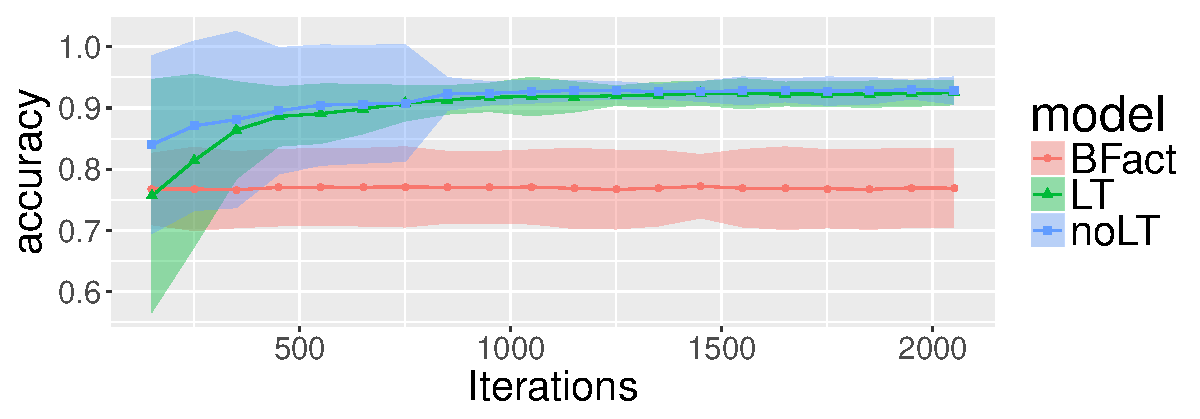
\includegraphics[width = 0.3\textwidth]{/Users/cdawson/src/hdp_hmm_lt/experiment/visualizations/fig/cocktail/hsmm/noise_a1b1/cp_0/accuracy}
  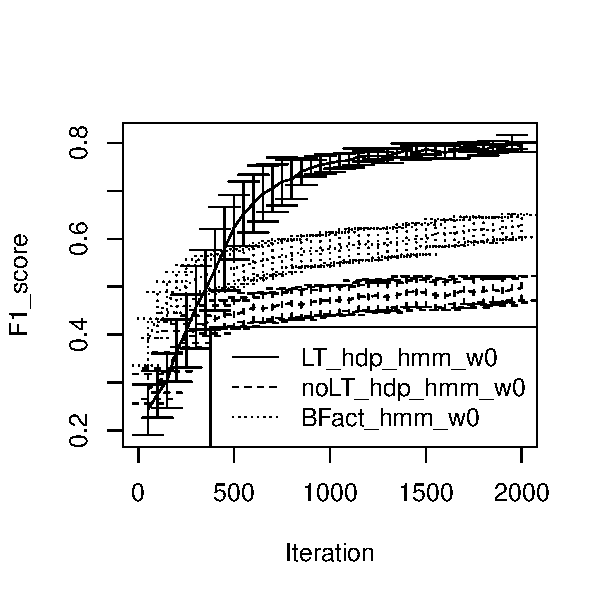
\includegraphics[width = 0.3\textwidth]{/Users/cdawson/src/hdp_hmm_lt/experiment/visualizations/fig/cocktail/hsmm/noise_a1b1/cp_0/F1_score}
  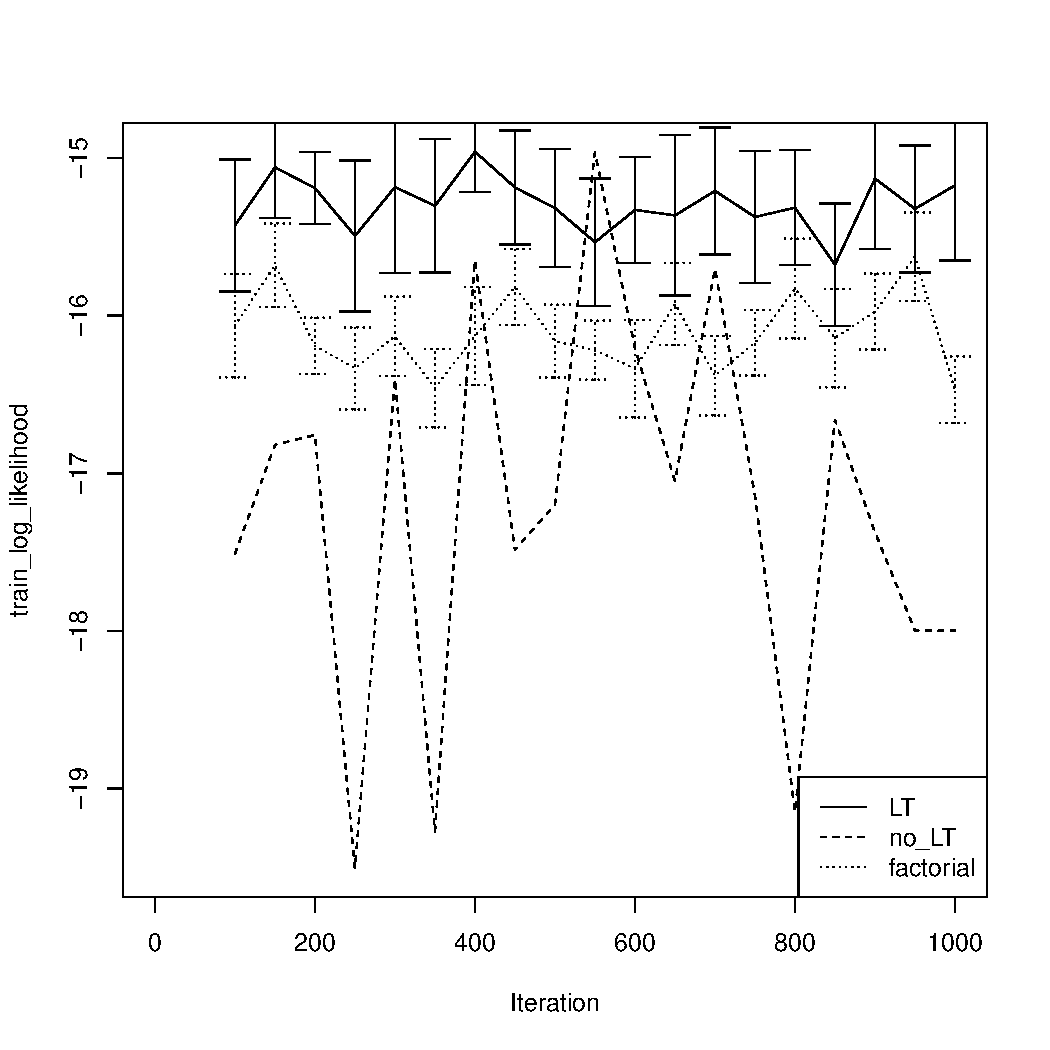
\includegraphics[width = 0.3\textwidth]{/Users/cdawson/src/hdp_hmm_lt/experiment/visualizations/fig/cocktail/hsmm/noise_a1b1/cp_0/train_log_likelihood}
  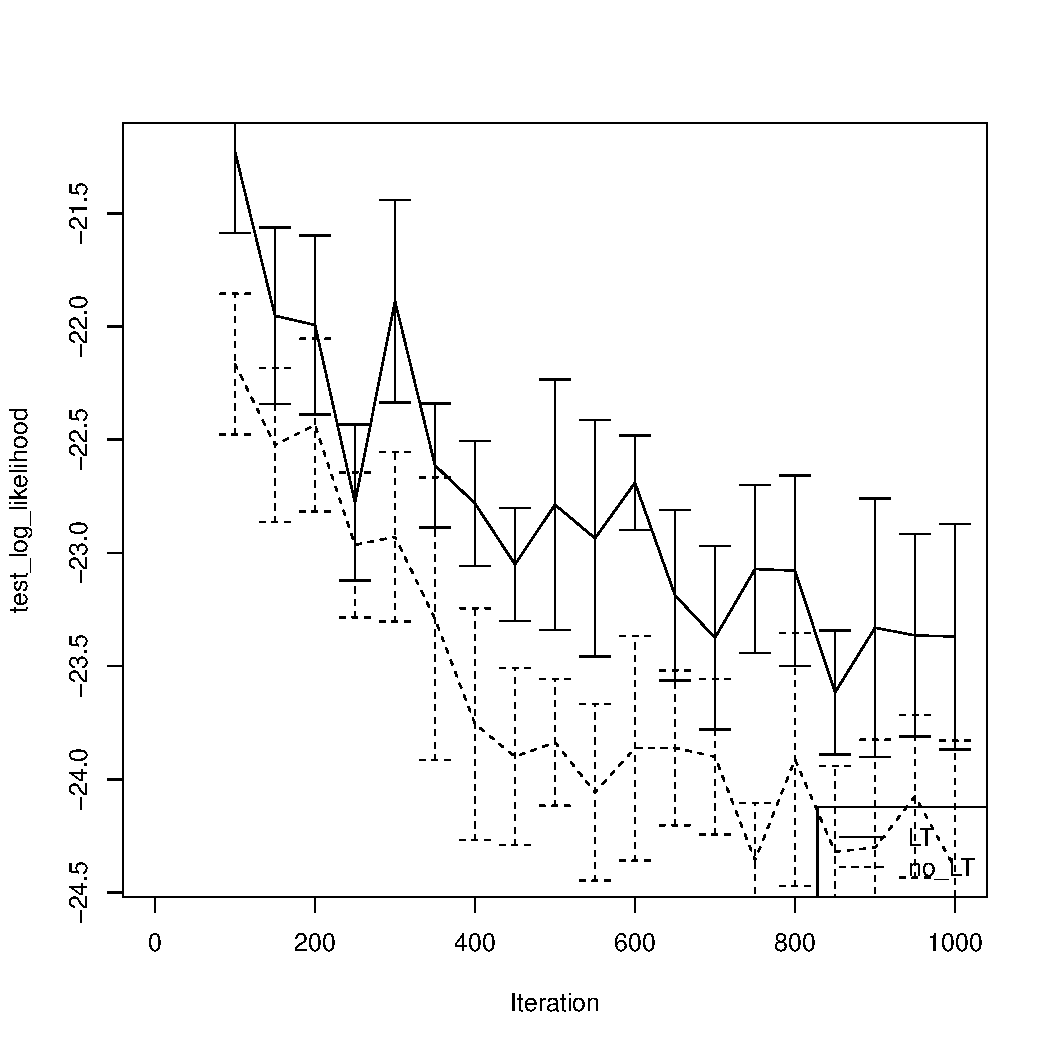
\includegraphics[width = 0.3\textwidth]{/Users/cdawson/src/hdp_hmm_lt/experiment/visualizations/fig/cocktail/hsmm/noise_a1b1/cp_0/test_log_likelihood}
  \caption{Performance of the Factorial HMM, HDP-HMM, and HDP-HSMM on
    the Cocktail Party Data.  For the HDP models, metrics are averaged
  over 10 Gibbs runs, with error bars representing a 99\% confidence
  interval for the mean per iteration.  The first 100 iterations are
  excluded as burn-in.}
  \label{fig:cocktail-results}
\end{figure}

\begin{figure}[tb]
  \centering
  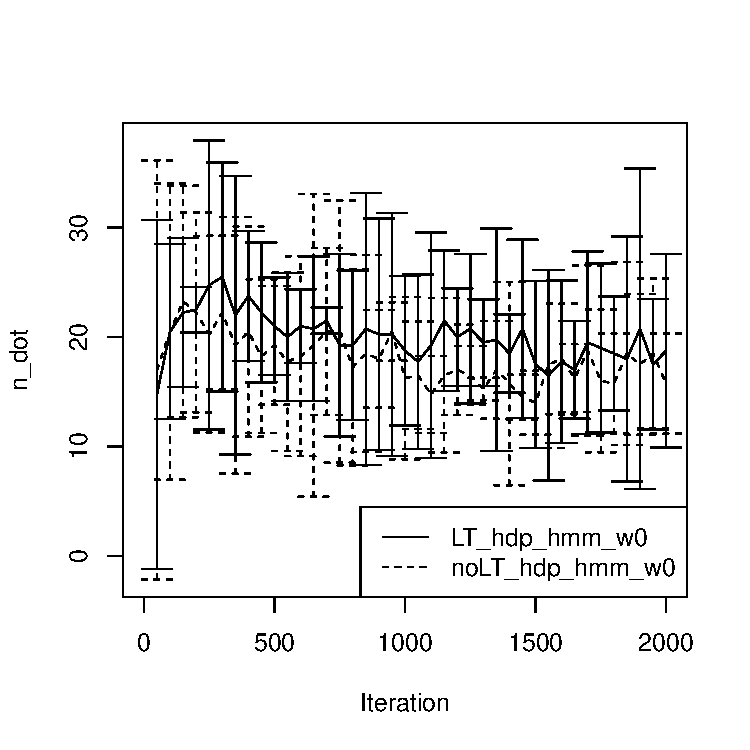
\includegraphics[width = 0.3\textwidth]{/Users/cdawson/src/hdp_hmm_lt/experiment/visualizations/fig/cocktail/hsmm/noise_a1b1/cp_0/n_dot}
  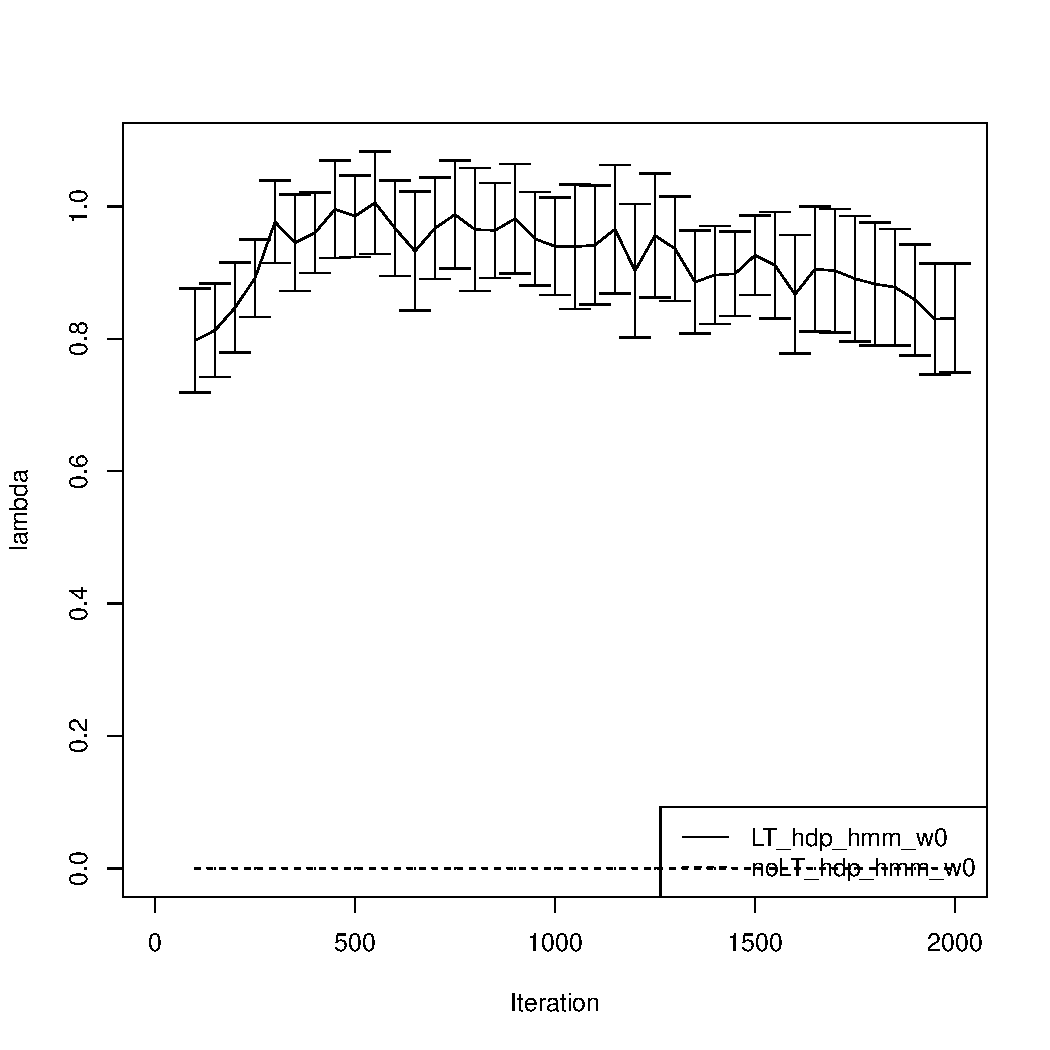
\includegraphics[width = 0.3\textwidth]{/Users/cdawson/src/hdp_hmm_lt/experiment/visualizations/fig/cocktail/hsmm/noise_a1b1/cp_0/lambda}
  \caption{Number of states used on the training data (top), and
    learned decay rate for the LT model (bottom) on the cocktail data. The first 100
    iterations are excluded.}
  \label{fig:sparsity}
\end{figure}

% \begin{figure}[tb]
%   \centering
%   \includegraphics[width = 0.3\textwidth]{/Users/cdawson/src/hdp_hmm_lt/experiment/visualizations/fig/cocktail/hsmm/noise_a1b1/cp_0/thetastar}
%   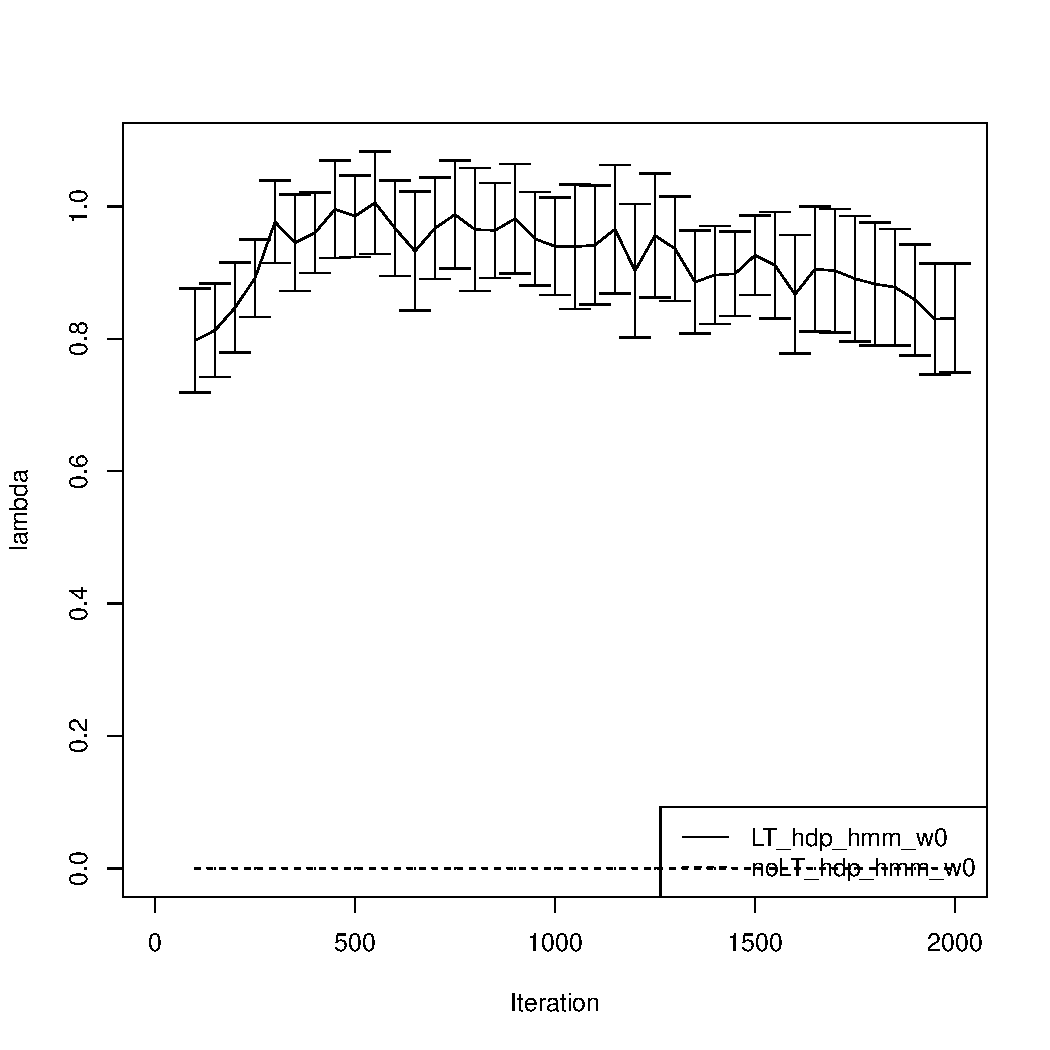
\includegraphics[width = 0.3\textwidth]{/Users/cdawson/src/hdp_hmm_lt/experiment/visualizations/fig/cocktail/hsmm/noise_a1b1/cp_0/lambda}
%   \caption{Number of states used on the training data (top), and
%     learned decay rate for the LT model (bottom) on the cocktail data. The first 100
%     iterations are excluded.}
%   \label{fig:sparsity}
% \end{figure}

\subsection{Synthetic Data Without Local Transitions}
\label{sec:synth-data-without}

We also generated data from an ordinary HDP-HMM, with no local
transition property, in order to investigate the performance of our
model in a case where the data did not have the key property that its
prior equipped it to discover.  The results are in
Figs. \ref{fig:synthetic-results} and \ref{fig:synthetic-sparsity}.
The model with local transitions performs equally well to the simpler
model in terms of ground truth labels, and in terms of marginal
likelihood on both the training and test set, appears to peform
somewhat better.

\begin{figure}[tb]
  \centering
  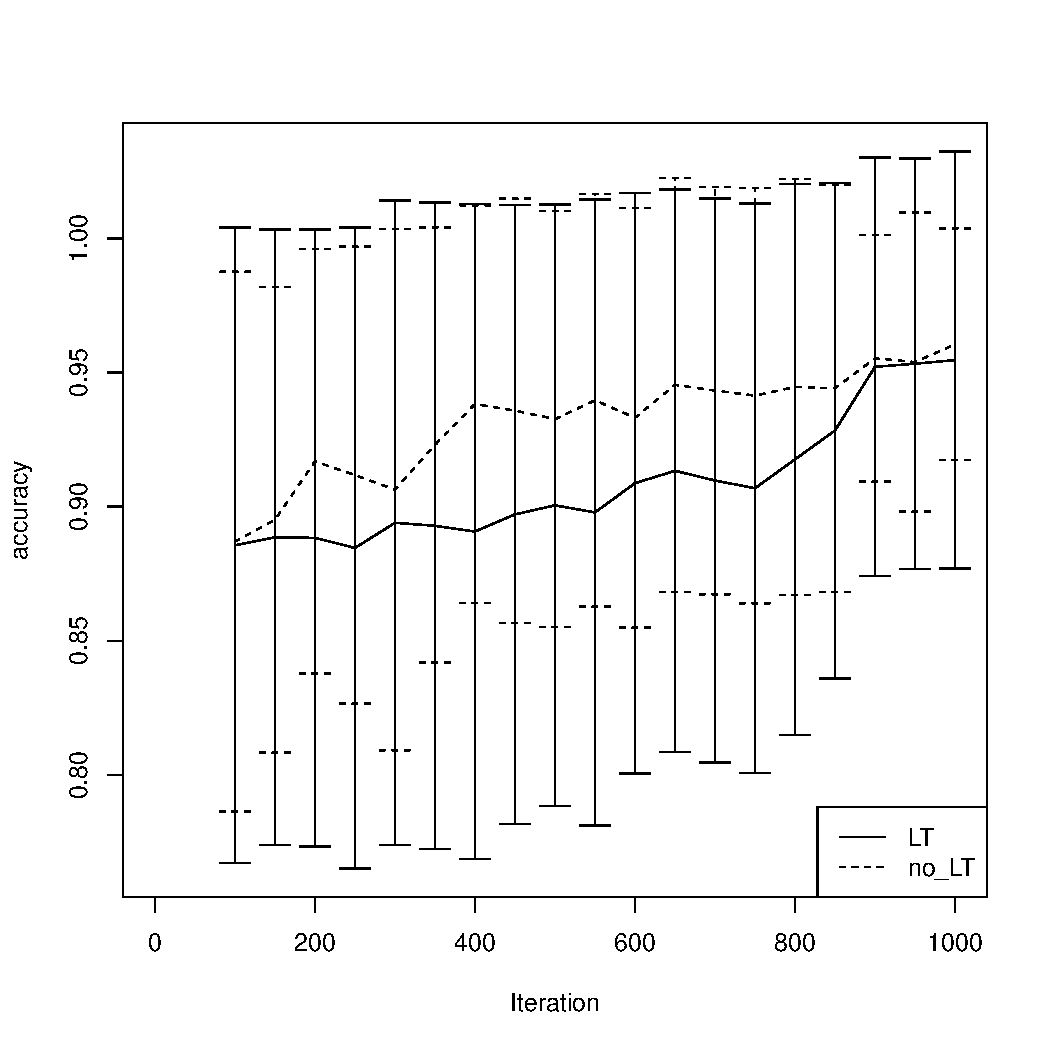
\includegraphics[width = 0.3\textwidth]{fig/synthetic/accuracy}
  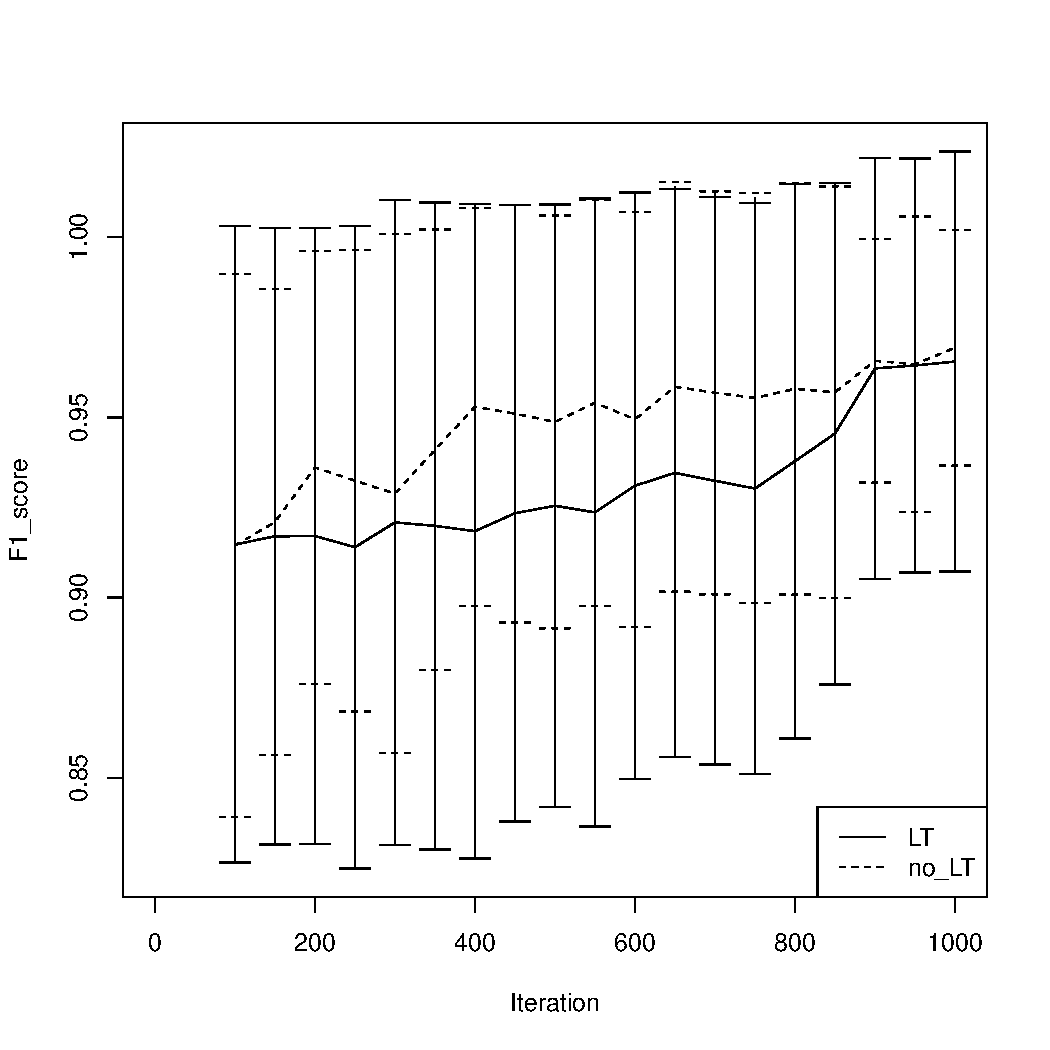
\includegraphics[width = 0.3\textwidth]{fig/synthetic/F1_score}
  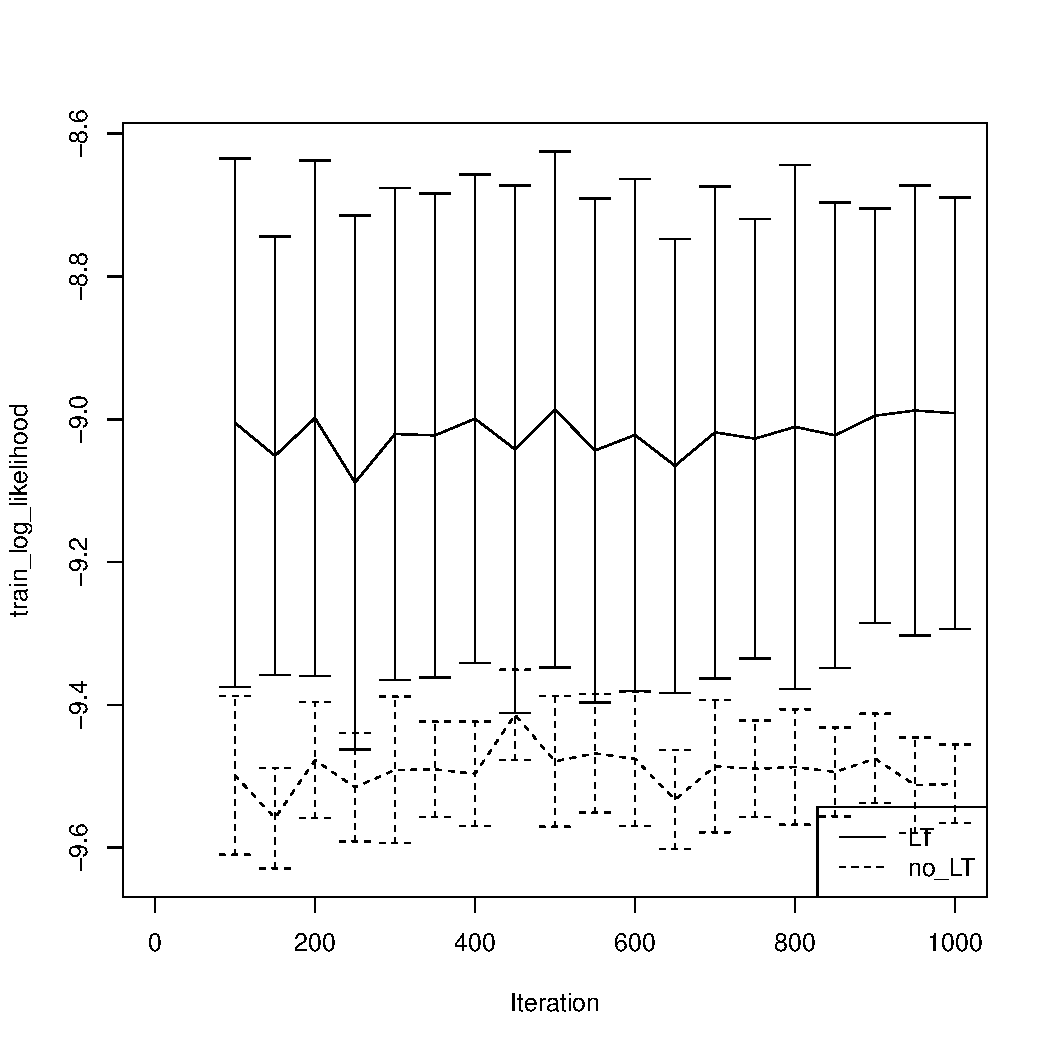
\includegraphics[width = 0.3\textwidth]{fig/synthetic/train_log_likelihood}
  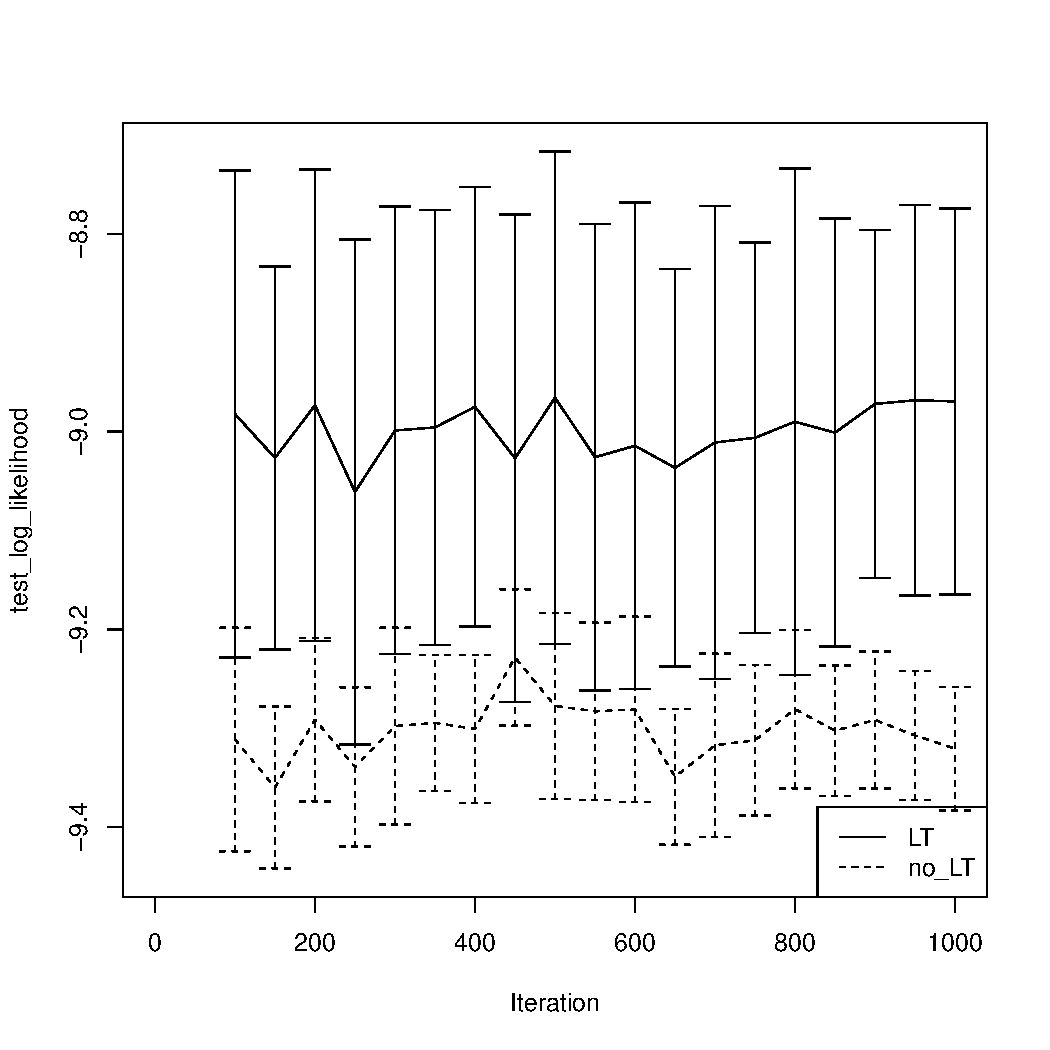
\includegraphics[width = 0.3\textwidth]{fig/synthetic/test_log_likelihood}
  \caption{Performance of the HDP-HMM with and without local transitions
    on data generated from an HDP-HMM without local transistions.}
  \label{fig:synthetic-results}
\end{figure}

\begin{figure}[tb]
  \centering
  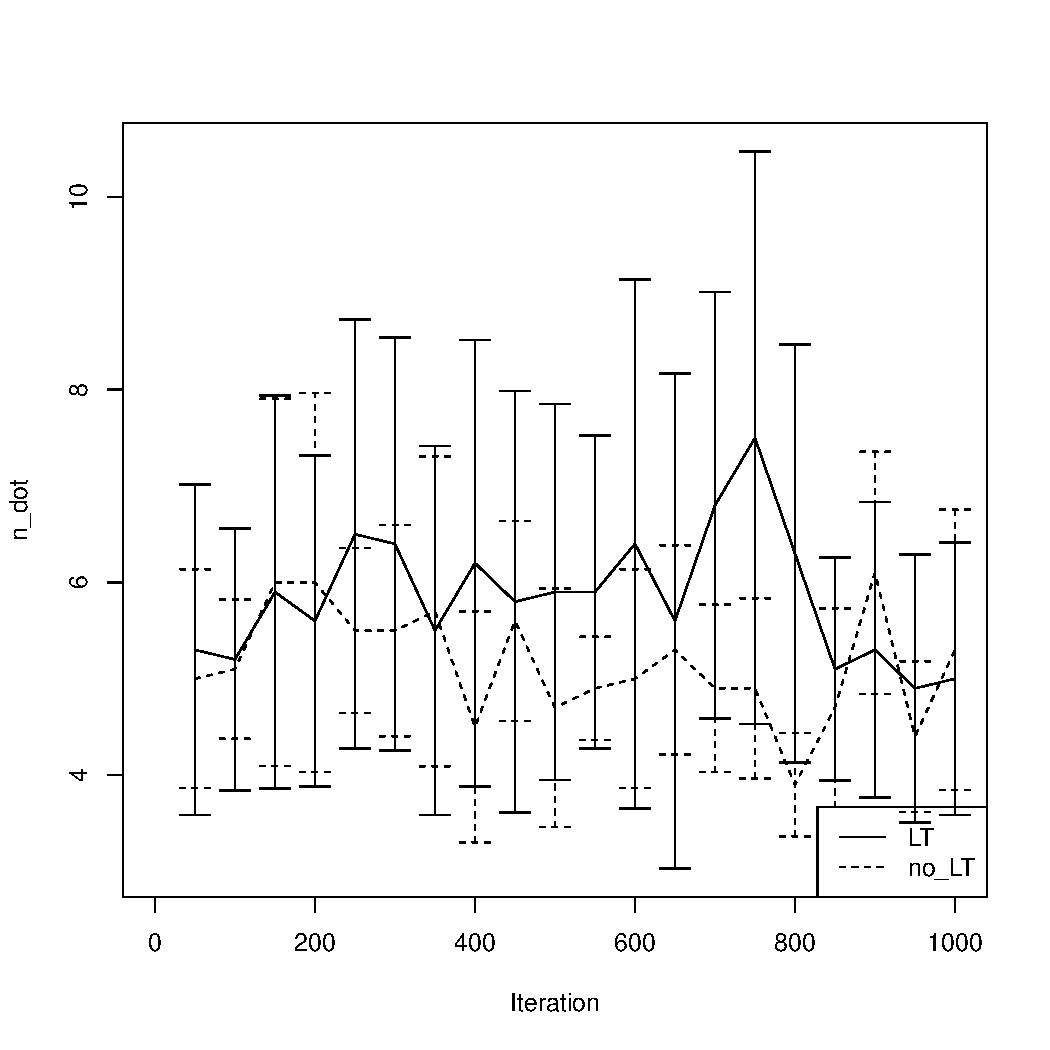
\includegraphics[width = 0.3\textwidth]{fig/synthetic/n_dot}
  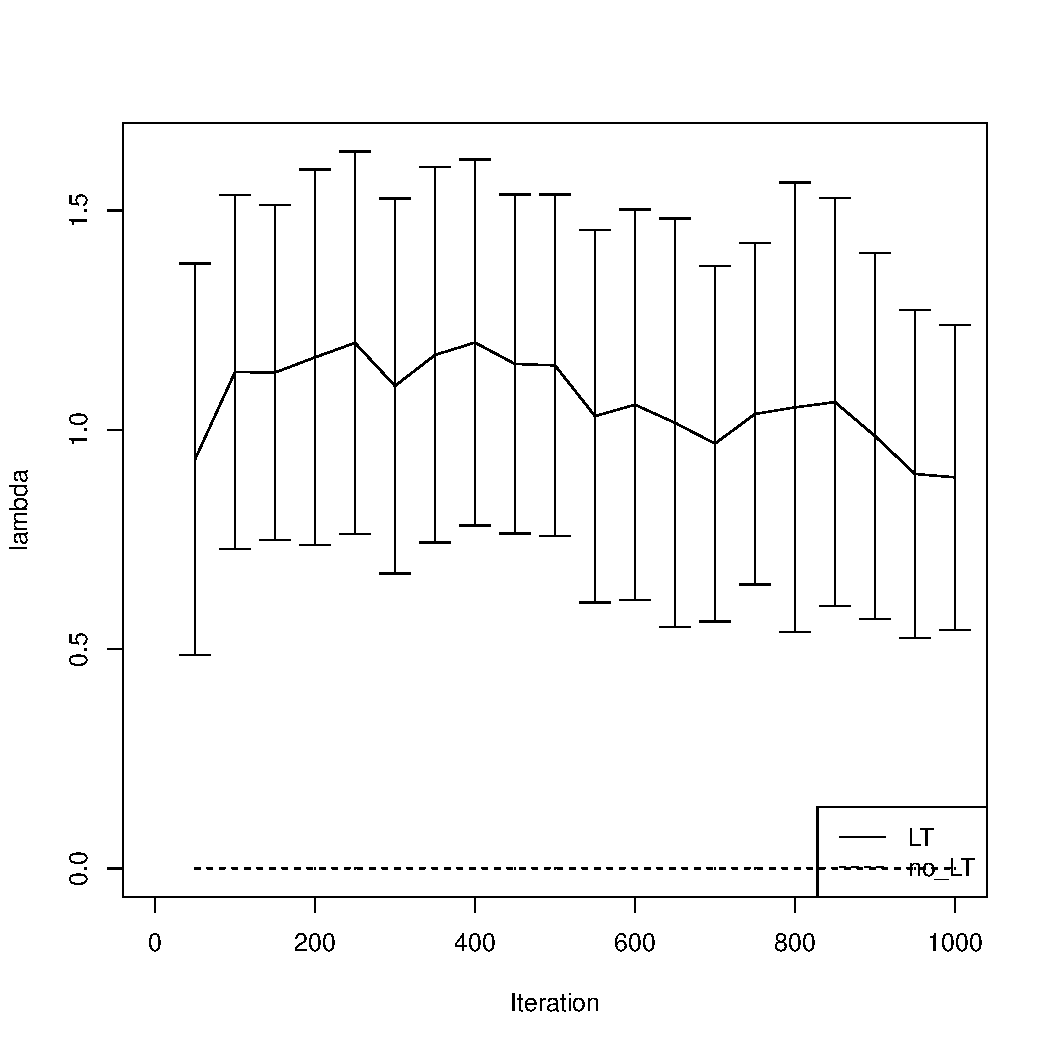
\includegraphics[width = 0.3\textwidth]{fig/synthetic/lambda}
  \caption{Number of states used on the training data (top), and
    learned decay rate for the LT model (bottom) on the HDP-HMM data. The first 100
    iterations are excluded.}
  \label{fig:synthetic-sparsity}
\end{figure}
